\documentclass[1p]{elsarticle_modified}
%\bibliographystyle{elsarticle-num}

%\usepackage[colorlinks]{hyperref}
%\usepackage{abbrmath_seonhwa} %\Abb, \Ascr, \Acal ,\Abf, \Afrak
\usepackage{amsfonts}
\usepackage{amssymb}
\usepackage{amsmath}
\usepackage{amsthm}
\usepackage{scalefnt}
\usepackage{amsbsy}
\usepackage{kotex}
\usepackage{caption}
\usepackage{subfig}
\usepackage{color}
\usepackage{graphicx}
\usepackage{xcolor} %% white, black, red, green, blue, cyan, magenta, yellow
\usepackage{float}
\usepackage{setspace}
\usepackage{hyperref}

\usepackage{tikz}
\usetikzlibrary{arrows}

\usepackage{multirow}
\usepackage{array} % fixed length table
\usepackage{hhline}

%%%%%%%%%%%%%%%%%%%%%
\makeatletter
\renewcommand*\env@matrix[1][\arraystretch]{%
	\edef\arraystretch{#1}%
	\hskip -\arraycolsep
	\let\@ifnextchar\new@ifnextchar
	\array{*\c@MaxMatrixCols c}}
\makeatother %https://tex.stackexchange.com/questions/14071/how-can-i-increase-the-line-spacing-in-a-matrix
%%%%%%%%%%%%%%%

\usepackage[normalem]{ulem}

\newcommand{\msout}[1]{\ifmmode\text{\sout{\ensuremath{#1}}}\else\sout{#1}\fi}
%SOURCE: \msout is \stkout macro in https://tex.stackexchange.com/questions/20609/strikeout-in-math-mode

\newcommand{\cancel}[1]{
	\ifmmode
	{\color{red}\msout{#1}}
	\else
	{\color{red}\sout{#1}}
	\fi
}

\newcommand{\add}[1]{
	{\color{blue}\uwave{#1}}
}

\newcommand{\replace}[2]{
	\ifmmode
	{\color{red}\msout{#1}}{\color{blue}\uwave{#2}}
	\else
	{\color{red}\sout{#1}}{\color{blue}\uwave{#2}}
	\fi
}

\newcommand{\Sol}{\mathcal{S}} %segment
\newcommand{\D}{D} %diagram
\newcommand{\A}{\mathcal{A}} %arc


%%%%%%%%%%%%%%%%%%%%%%%%%%%%%5 test

\def\sl{\operatorname{\textup{SL}}(2,\Cbb)}
\def\psl{\operatorname{\textup{PSL}}(2,\Cbb)}
\def\quan{\mkern 1mu \triangleright \mkern 1mu}

\theoremstyle{definition}
\newtheorem{thm}{Theorem}[section]
\newtheorem{prop}[thm]{Proposition}
\newtheorem{lem}[thm]{Lemma}
\newtheorem{ques}[thm]{Question}
\newtheorem{cor}[thm]{Corollary}
\newtheorem{defn}[thm]{Definition}
\newtheorem{exam}[thm]{Example}
\newtheorem{rmk}[thm]{Remark}
\newtheorem{alg}[thm]{Algorithm}

\newcommand{\I}{\sqrt{-1}}
\begin{document}

%\begin{frontmatter}
%
%\title{Boundary parabolic representations of knots up to 8 crossings}
%
%%% Group authors per affiliation:
%\author{Yunhi Cho} 
%\address{Department of Mathematics, University of Seoul, Seoul, Korea}
%\ead{yhcho@uos.ac.kr}
%
%
%\author{Seonhwa Kim} %\fnref{s_kim}}
%\address{Center for Geometry and Physics, Institute for Basic Science, Pohang, 37673, Korea}
%\ead{ryeona17@ibs.re.kr}
%
%\author{Hyuk Kim}
%\address{Department of Mathematical Sciences, Seoul National University, Seoul 08826, Korea}
%\ead{hyukkim@snu.ac.kr}
%
%\author{Seokbeom Yoon}
%\address{Department of Mathematical Sciences, Seoul National University, Seoul, 08826,  Korea}
%\ead{sbyoon15@snu.ac.kr}
%
%\begin{abstract}
%We find all boundary parabolic representation of knots up to 8 crossings.
%
%\end{abstract}
%\begin{keyword}
%    \MSC[2010] 57M25 
%\end{keyword}
%
%\end{frontmatter}

%\linenumbers
%\tableofcontents
%
\newcommand\colored[1]{\textcolor{white}{\rule[-0.35ex]{0.8em}{1.4ex}}\kern-0.8em\color{red} #1}%
%\newcommand\colored[1]{\textcolor{white}{ #1}\kern-2.17ex	\textcolor{white}{ #1}\kern-1.81ex	\textcolor{white}{ #1}\kern-2.15ex\color{red}#1	}

{\Large $\underline{12a_{0133}~(K12a_{0133})}$}

\setlength{\tabcolsep}{10pt}
\renewcommand{\arraystretch}{1.6}
\vspace{1cm}\begin{tabular}{m{100pt}>{\centering\arraybackslash}m{274pt}}
\multirow{5}{120pt}{
	\centering
	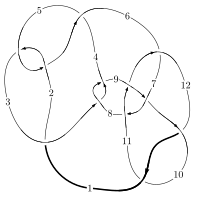
\includegraphics[width=112pt]{../../../GIT/diagram.site/Diagrams/png/934_12a_0133.png}\\
\ \ \ A knot diagram\footnotemark}&
\allowdisplaybreaks
\textbf{Linearized knot diagam} \\
\cline{2-2}
 &
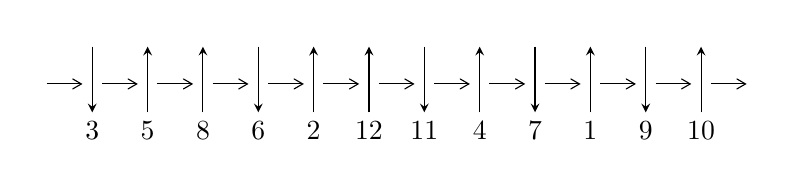
\begin{tikzpicture}[x=20pt, y=17pt]
	% nodes
	\node (C0) at (0, 0) {};
	\node (C1) at (1, 0) {};
	\node (C1U) at (1, +1) {};
	\node (C1D) at (1, -1) {3};

	\node (C2) at (2, 0) {};
	\node (C2U) at (2, +1) {};
	\node (C2D) at (2, -1) {5};

	\node (C3) at (3, 0) {};
	\node (C3U) at (3, +1) {};
	\node (C3D) at (3, -1) {8};

	\node (C4) at (4, 0) {};
	\node (C4U) at (4, +1) {};
	\node (C4D) at (4, -1) {6};

	\node (C5) at (5, 0) {};
	\node (C5U) at (5, +1) {};
	\node (C5D) at (5, -1) {2};

	\node (C6) at (6, 0) {};
	\node (C6U) at (6, +1) {};
	\node (C6D) at (6, -1) {12};

	\node (C7) at (7, 0) {};
	\node (C7U) at (7, +1) {};
	\node (C7D) at (7, -1) {11};

	\node (C8) at (8, 0) {};
	\node (C8U) at (8, +1) {};
	\node (C8D) at (8, -1) {4};

	\node (C9) at (9, 0) {};
	\node (C9U) at (9, +1) {};
	\node (C9D) at (9, -1) {7};

	\node (C10) at (10, 0) {};
	\node (C10U) at (10, +1) {};
	\node (C10D) at (10, -1) {1};

	\node (C11) at (11, 0) {};
	\node (C11U) at (11, +1) {};
	\node (C11D) at (11, -1) {9};

	\node (C12) at (12, 0) {};
	\node (C12U) at (12, +1) {};
	\node (C12D) at (12, -1) {10};
	\node (C13) at (13, 0) {};

	% arrows
	\draw[->,>={angle 60}]
	(C0) edge (C1) (C1) edge (C2) (C2) edge (C3) (C3) edge (C4) (C4) edge (C5) (C5) edge (C6) (C6) edge (C7) (C7) edge (C8) (C8) edge (C9) (C9) edge (C10) (C10) edge (C11) (C11) edge (C12) (C12) edge (C13) ;	\draw[->,>=stealth]
	(C1U) edge (C1D) (C2D) edge (C2U) (C3D) edge (C3U) (C4U) edge (C4D) (C5D) edge (C5U) (C6D) edge (C6U) (C7U) edge (C7D) (C8D) edge (C8U) (C9U) edge (C9D) (C10D) edge (C10U) (C11U) edge (C11D) (C12D) edge (C12U) ;
	\end{tikzpicture} \\
\hhline{~~} \\& 
\textbf{Solving Sequence} \\ \cline{2-2} 
 &
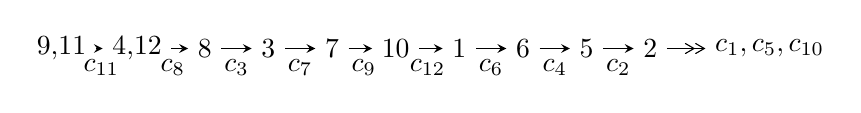
\begin{tikzpicture}[x=23pt, y=7pt]
	% node
	\node (A0) at (-1/8, 0) {9,11};
	\node (A1) at (17/16, 0) {4,12};
	\node (A2) at (17/8, 0) {8};
	\node (A3) at (25/8, 0) {3};
	\node (A4) at (33/8, 0) {7};
	\node (A5) at (41/8, 0) {10};
	\node (A6) at (49/8, 0) {1};
	\node (A7) at (57/8, 0) {6};
	\node (A8) at (65/8, 0) {5};
	\node (A9) at (73/8, 0) {2};
	\node (C1) at (1/2, -1) {$c_{11}$};
	\node (C2) at (13/8, -1) {$c_{8}$};
	\node (C3) at (21/8, -1) {$c_{3}$};
	\node (C4) at (29/8, -1) {$c_{7}$};
	\node (C5) at (37/8, -1) {$c_{9}$};
	\node (C6) at (45/8, -1) {$c_{12}$};
	\node (C7) at (53/8, -1) {$c_{6}$};
	\node (C8) at (61/8, -1) {$c_{4}$};
	\node (C9) at (69/8, -1) {$c_{2}$};
	\node (A10) at (11, 0) {$c_{1},c_{5},c_{10}$};

	% edge
	\draw[->,>=stealth]	
	(A0) edge (A1) (A1) edge (A2) (A2) edge (A3) (A3) edge (A4) (A4) edge (A5) (A5) edge (A6) (A6) edge (A7) (A7) edge (A8) (A8) edge (A9) ;
	\draw[->>,>={angle 60}]	
	(A9) edge (A10);
\end{tikzpicture} \\ 

\end{tabular} \\

\footnotetext{
The image of knot diagram is generated by the software ``\textbf{Draw programme}" developed by Andrew Bartholomew(\url{http://www.layer8.co.uk/maths/draw/index.htm\#Running-draw}), where we modified some parts for our purpose(\url{https://github.com/CATsTAILs/LinksPainter}).
}\phantom \\ \newline 
\centering \textbf{Ideals for irreducible components\footnotemark of $X_{\text{par}}$} 
 
\begin{align*}
I^u_{1}&=\langle 
-1.85504\times10^{788} u^{124}+3.67648\times10^{789} u^{123}+\cdots+1.84177\times10^{788} b-7.07747\times10^{788},\\
\phantom{I^u_{1}}&\phantom{= \langle  }-2.43301\times10^{788} u^{124}+5.11381\times10^{789} u^{123}+\cdots+9.20887\times10^{787} a+7.40748\times10^{788},\\
\phantom{I^u_{1}}&\phantom{= \langle  }u^{125}-21 u^{124}+\cdots-3 u+1\rangle \\
I^u_{2}&=\langle 
- u^5 b+2 u^5+u^3 b-3 u^3+b^2- b u- b+3 u+1,\;a,\;u^6- u^5- u^4+2 u^3- u+1\rangle \\
\\
\end{align*}
\raggedright * 2 irreducible components of $\dim_{\mathbb{C}}=0$, with total 137 representations.\\
\footnotetext{All coefficients of polynomials are rational numbers. But the coefficients are sometimes approximated in decimal forms when there is not enough margin.}
\newpage
\renewcommand{\arraystretch}{1}
\centering \section*{I. $I^u_{1}= \langle -1.86\times10^{788} u^{124}+3.68\times10^{789} u^{123}+\cdots+1.84\times10^{788} b-7.08\times10^{788},\;-2.43\times10^{788} u^{124}+5.11\times10^{789} u^{123}+\cdots+9.21\times10^{787} a+7.41\times10^{788},\;u^{125}-21 u^{124}+\cdots-3 u+1 \rangle$}
\flushleft \textbf{(i) Arc colorings}\\
\begin{tabular}{m{7pt} m{180pt} m{7pt} m{180pt} }
\flushright $a_{9}=$&$\begin{pmatrix}0\\u\end{pmatrix}$ \\
\flushright $a_{11}=$&$\begin{pmatrix}1\\0\end{pmatrix}$ \\
\flushright $a_{4}=$&$\begin{pmatrix}2.64203 u^{124}-55.5313 u^{123}+\cdots+19.1899 u-8.04385\\1.00720 u^{124}-19.9616 u^{123}+\cdots+5.57665 u+3.84275\end{pmatrix}$ \\
\flushright $a_{12}=$&$\begin{pmatrix}1\\u^2\end{pmatrix}$ \\
\flushright $a_{8}=$&$\begin{pmatrix}0.481862 u^{124}-11.4373 u^{123}+\cdots+6.21816 u-7.95654\\0.193276 u^{124}-3.35222 u^{123}+\cdots-2.51683 u+3.74346\end{pmatrix}$ \\
\flushright $a_{3}=$&$\begin{pmatrix}5.54735 u^{124}-116.372 u^{123}+\cdots+44.2277 u-12.9410\\0.987816 u^{124}-19.2874 u^{123}+\cdots+3.17753 u+5.56318\end{pmatrix}$ \\
\flushright $a_{7}=$&$\begin{pmatrix}0.675138 u^{124}-14.7895 u^{123}+\cdots+3.70134 u-4.21308\\0.193276 u^{124}-3.35222 u^{123}+\cdots-2.51683 u+3.74346\end{pmatrix}$ \\
\flushright $a_{10}=$&$\begin{pmatrix}-0.0738144 u^{124}+1.46614 u^{123}+\cdots-0.540455 u+1.43814\\0.581451 u^{124}-12.1584 u^{123}+\cdots+2.87063 u-1.11559\end{pmatrix}$ \\
\flushright $a_{1}=$&$\begin{pmatrix}-0.0738144 u^{124}+1.46614 u^{123}+\cdots-0.540455 u+1.43814\\-0.669841 u^{124}+14.0038 u^{123}+\cdots-3.04870 u+1.19955\end{pmatrix}$ \\
\flushright $a_{6}=$&$\begin{pmatrix}0.110132 u^{124}-3.63794 u^{123}+\cdots+3.70815 u-7.34491\\-0.00891814 u^{124}+0.907468 u^{123}+\cdots-4.09245 u+4.45700\end{pmatrix}$ \\
\flushright $a_{5}=$&$\begin{pmatrix}6.04837 u^{124}-126.686 u^{123}+\cdots+46.7051 u-14.3744\\1.25389 u^{124}-24.7312 u^{123}+\cdots+4.66284 u+5.75382\end{pmatrix}$ \\
\flushright $a_{2}=$&$\begin{pmatrix}1.97982 u^{124}-43.5856 u^{123}+\cdots+16.2112 u-16.0378\\-1.16126 u^{124}+25.5464 u^{123}+\cdots-13.1425 u+10.4296\end{pmatrix}$\\&\end{tabular}
\flushleft \textbf{(ii) Obstruction class $= -1$}\\~\\
\flushleft \textbf{(iii) Cusp Shapes $= 2.99618 u^{124}-67.3888 u^{123}+\cdots+57.9690 u-28.9195$}\\~\\
\newpage\renewcommand{\arraystretch}{1}
\flushleft \textbf{(iv) u-Polynomials at the component}\newline \\
\begin{tabular}{m{50pt}|m{274pt}}
Crossings & \hspace{64pt}u-Polynomials at each crossing \\
\hline $$\begin{aligned}c_{1},c_{4}\end{aligned}$$&$\begin{aligned}
&u^{125}+41 u^{124}+\cdots-145 u-1
\end{aligned}$\\
\hline $$\begin{aligned}c_{2},c_{5}\end{aligned}$$&$\begin{aligned}
&u^{125}+7 u^{124}+\cdots-9 u-1
\end{aligned}$\\
\hline $$\begin{aligned}c_{3},c_{8}\end{aligned}$$&$\begin{aligned}
&u^{125}- u^{124}+\cdots+20480 u-4096
\end{aligned}$\\
\hline $$\begin{aligned}c_{6}\end{aligned}$$&$\begin{aligned}
&u^{125}+9 u^{124}+\cdots+391375 u+25489
\end{aligned}$\\
\hline $$\begin{aligned}c_{7}\end{aligned}$$&$\begin{aligned}
&u^{125}+3 u^{124}+\cdots-6561489 u+604147
\end{aligned}$\\
\hline $$\begin{aligned}c_{9}\end{aligned}$$&$\begin{aligned}
&u^{125}-9 u^{124}+\cdots-3 u+1
\end{aligned}$\\
\hline $$\begin{aligned}c_{10},c_{12}\end{aligned}$$&$\begin{aligned}
&u^{125}+3 u^{124}+\cdots+17 u-1
\end{aligned}$\\
\hline $$\begin{aligned}c_{11}\end{aligned}$$&$\begin{aligned}
&u^{125}-21 u^{124}+\cdots-3 u+1
\end{aligned}$\\
\hline
\end{tabular}\\~\\
\newpage\renewcommand{\arraystretch}{1}
\flushleft \textbf{(v) Riley Polynomials at the component}\newline \\
\begin{tabular}{m{50pt}|m{274pt}}
Crossings & \hspace{64pt}Riley Polynomials at each crossing \\
\hline $$\begin{aligned}c_{1},c_{4}\end{aligned}$$&$\begin{aligned}
&y^{125}+93 y^{124}+\cdots+5099 y-1
\end{aligned}$\\
\hline $$\begin{aligned}c_{2},c_{5}\end{aligned}$$&$\begin{aligned}
&y^{125}+41 y^{124}+\cdots-145 y-1
\end{aligned}$\\
\hline $$\begin{aligned}c_{3},c_{8}\end{aligned}$$&$\begin{aligned}
&y^{125}-65 y^{124}+\cdots+301989888 y-16777216
\end{aligned}$\\
\hline $$\begin{aligned}c_{6}\end{aligned}$$&$\begin{aligned}
&y^{125}-127 y^{124}+\cdots+36942460527 y-649689121
\end{aligned}$\\
\hline $$\begin{aligned}c_{7}\end{aligned}$$&$\begin{aligned}
&y^{125}-91 y^{124}+\cdots-24775319389441 y-364993597609
\end{aligned}$\\
\hline $$\begin{aligned}c_{9}\end{aligned}$$&$\begin{aligned}
&y^{125}+21 y^{124}+\cdots-9 y-1
\end{aligned}$\\
\hline $$\begin{aligned}c_{10},c_{12}\end{aligned}$$&$\begin{aligned}
&y^{125}-83 y^{124}+\cdots-17 y-1
\end{aligned}$\\
\hline $$\begin{aligned}c_{11}\end{aligned}$$&$\begin{aligned}
&y^{125}-3 y^{124}+\cdots-17 y-1
\end{aligned}$\\
\hline
\end{tabular}\\~\\
\newpage\flushleft \textbf{(vi) Complex Volumes and Cusp Shapes}
$$\begin{array}{c|c|c}  
\text{Solutions to }I^u_{1}& \I (\text{vol} + \sqrt{-1}CS) & \text{Cusp shape}\\
 \hline 
\begin{aligned}
u &= -0.655767 + 0.724024 I \\
a &= \phantom{-}0.33434 + 1.55566 I \\
b &= \phantom{-}0.447793 - 1.297880 I\end{aligned}
 & \phantom{-}6.22986 + 11.45440 I & \phantom{-0.000000 } 0 \\ \hline\begin{aligned}
u &= -0.655767 - 0.724024 I \\
a &= \phantom{-}0.33434 - 1.55566 I \\
b &= \phantom{-}0.447793 + 1.297880 I\end{aligned}
 & \phantom{-}6.22986 - 11.45440 I & \phantom{-0.000000 } 0 \\ \hline\begin{aligned}
u &= \phantom{-}0.800249 + 0.648673 I \\
a &= -0.435423 - 0.783872 I \\
b &= \phantom{-}0.0861307 + 0.1080150 I\end{aligned}
 & \phantom{-}1.30610 - 5.13081 I & \phantom{-0.000000 } 0 \\ \hline\begin{aligned}
u &= \phantom{-}0.800249 - 0.648673 I \\
a &= -0.435423 + 0.783872 I \\
b &= \phantom{-}0.0861307 - 0.1080150 I\end{aligned}
 & \phantom{-}1.30610 + 5.13081 I & \phantom{-0.000000 } 0 \\ \hline\begin{aligned}
u &= -0.812584 + 0.469650 I \\
a &= \phantom{-}0.404002 - 0.446533 I \\
b &= \phantom{-}0.205603 - 0.077552 I\end{aligned}
 & -1.40641 + 1.21884 I & \phantom{-0.000000 } 0 \\ \hline\begin{aligned}
u &= -0.812584 - 0.469650 I \\
a &= \phantom{-}0.404002 + 0.446533 I \\
b &= \phantom{-}0.205603 + 0.077552 I\end{aligned}
 & -1.40641 - 1.21884 I & \phantom{-0.000000 } 0 \\ \hline\begin{aligned}
u &= -0.556208 + 0.736230 I \\
a &= -0.28352 - 1.68148 I \\
b &= -0.372160 + 1.230560 I\end{aligned}
 & \phantom{-}7.45341 + 5.28303 I & \phantom{-0.000000 } 0 \\ \hline\begin{aligned}
u &= -0.556208 - 0.736230 I \\
a &= -0.28352 + 1.68148 I \\
b &= -0.372160 - 1.230560 I\end{aligned}
 & \phantom{-}7.45341 - 5.28303 I & \phantom{-0.000000 } 0 \\ \hline\begin{aligned}
u &= -0.906987 + 0.030403 I \\
a &= \phantom{-}0.519200 - 0.675115 I \\
b &= -0.025247 - 0.165447 I\end{aligned}
 & -3.11701 + 0.35524 I & \phantom{-0.000000 } 0 \\ \hline\begin{aligned}
u &= -0.906987 - 0.030403 I \\
a &= \phantom{-}0.519200 + 0.675115 I \\
b &= -0.025247 + 0.165447 I\end{aligned}
 & -3.11701 - 0.35524 I & \phantom{-0.000000 } 0\\
 \hline 
 \end{array}$$\newpage$$\begin{array}{c|c|c}  
\text{Solutions to }I^u_{1}& \I (\text{vol} + \sqrt{-1}CS) & \text{Cusp shape}\\
 \hline 
\begin{aligned}
u &= \phantom{-}1.149600 + 0.349509 I \\
a &= -0.535012 + 0.432272 I \\
b &= \phantom{-}0.078999 - 0.123440 I\end{aligned}
 & \phantom{-}0.35042 - 8.49800 I & \phantom{-0.000000 } 0 \\ \hline\begin{aligned}
u &= \phantom{-}1.149600 - 0.349509 I \\
a &= -0.535012 - 0.432272 I \\
b &= \phantom{-}0.078999 + 0.123440 I\end{aligned}
 & \phantom{-}0.35042 + 8.49800 I & \phantom{-0.000000 } 0 \\ \hline\begin{aligned}
u &= \phantom{-}0.601239 + 0.510683 I \\
a &= -0.62073 + 1.55220 I \\
b &= \phantom{-}0.094233 - 1.338300 I\end{aligned}
 & \phantom{-}3.00041 - 8.24027 I & \phantom{-0.000000 } 0 \\ \hline\begin{aligned}
u &= \phantom{-}0.601239 - 0.510683 I \\
a &= -0.62073 - 1.55220 I \\
b &= \phantom{-}0.094233 + 1.338300 I\end{aligned}
 & \phantom{-}3.00041 + 8.24027 I & \phantom{-0.000000 } 0 \\ \hline\begin{aligned}
u &= -0.874574 + 0.851604 I \\
a &= -0.310901 - 0.625158 I \\
b &= -1.21137 + 2.18977 I\end{aligned}
 & -1.140860 + 0.185574 I & \phantom{-0.000000 } 0 \\ \hline\begin{aligned}
u &= -0.874574 - 0.851604 I \\
a &= -0.310901 + 0.625158 I \\
b &= -1.21137 - 2.18977 I\end{aligned}
 & -1.140860 - 0.185574 I & \phantom{-0.000000 } 0 \\ \hline\begin{aligned}
u &= -0.081636 + 0.769248 I \\
a &= -0.36800 + 1.57288 I \\
b &= \phantom{-}0.83539 - 1.84910 I\end{aligned}
 & \phantom{-}4.79797 + 5.99082 I & \phantom{-0.000000 } 0 \\ \hline\begin{aligned}
u &= -0.081636 - 0.769248 I \\
a &= -0.36800 - 1.57288 I \\
b &= \phantom{-}0.83539 + 1.84910 I\end{aligned}
 & \phantom{-}4.79797 - 5.99082 I & \phantom{-0.000000 } 0 \\ \hline\begin{aligned}
u &= \phantom{-}1.079040 + 0.584332 I \\
a &= \phantom{-}0.456985 - 0.442276 I \\
b &= \phantom{-}0.69928 + 2.28590 I\end{aligned}
 & \phantom{-}2.34856 - 1.43127 I & \phantom{-0.000000 } 0 \\ \hline\begin{aligned}
u &= \phantom{-}1.079040 - 0.584332 I \\
a &= \phantom{-}0.456985 + 0.442276 I \\
b &= \phantom{-}0.69928 - 2.28590 I\end{aligned}
 & \phantom{-}2.34856 + 1.43127 I & \phantom{-0.000000 } 0\\
 \hline 
 \end{array}$$\newpage$$\begin{array}{c|c|c}  
\text{Solutions to }I^u_{1}& \I (\text{vol} + \sqrt{-1}CS) & \text{Cusp shape}\\
 \hline 
\begin{aligned}
u &= -0.012937 + 0.762843 I \\
a &= \phantom{-}0.34464 - 1.56179 I \\
b &= -0.79362 + 1.73569 I\end{aligned}
 & \phantom{-}5.39776 + 0.24395 I & \phantom{-0.000000 } 0 \\ \hline\begin{aligned}
u &= -0.012937 - 0.762843 I \\
a &= \phantom{-}0.34464 + 1.56179 I \\
b &= -0.79362 - 1.73569 I\end{aligned}
 & \phantom{-}5.39776 - 0.24395 I & \phantom{-0.000000 } 0 \\ \hline\begin{aligned}
u &= \phantom{-}0.465870 + 1.150330 I \\
a &= \phantom{-}0.562053 - 1.160690 I \\
b &= \phantom{-}0.54269 + 1.53375 I\end{aligned}
 & \phantom{-}12.64840 - 1.23482 I & \phantom{-0.000000 } 0 \\ \hline\begin{aligned}
u &= \phantom{-}0.465870 - 1.150330 I \\
a &= \phantom{-}0.562053 + 1.160690 I \\
b &= \phantom{-}0.54269 - 1.53375 I\end{aligned}
 & \phantom{-}12.64840 + 1.23482 I & \phantom{-0.000000 } 0 \\ \hline\begin{aligned}
u &= \phantom{-}0.709846 + 0.224075 I \\
a &= -0.52362 + 1.38728 I \\
b &= -0.080817 - 0.223298 I\end{aligned}
 & -2.63980 - 3.08960 I & \phantom{-0.000000 } 0 \\ \hline\begin{aligned}
u &= \phantom{-}0.709846 - 0.224075 I \\
a &= -0.52362 - 1.38728 I \\
b &= -0.080817 + 0.223298 I\end{aligned}
 & -2.63980 + 3.08960 I & \phantom{-0.000000 } 0 \\ \hline\begin{aligned}
u &= \phantom{-}0.514320 + 0.536168 I \\
a &= \phantom{-}0.57898 - 1.61891 I \\
b &= -0.187141 + 1.327970 I\end{aligned}
 & \phantom{-}3.99062 - 2.47202 I & \phantom{-0.000000 } 0 \\ \hline\begin{aligned}
u &= \phantom{-}0.514320 - 0.536168 I \\
a &= \phantom{-}0.57898 + 1.61891 I \\
b &= -0.187141 - 1.327970 I\end{aligned}
 & \phantom{-}3.99062 + 2.47202 I & \phantom{-0.000000 } 0 \\ \hline\begin{aligned}
u &= \phantom{-}0.720998 + 0.172200 I \\
a &= \phantom{-}0.469048 - 0.594384 I \\
b &= -0.36139 + 2.83331 I\end{aligned}
 & \phantom{-}2.22327 - 1.42836 I & \phantom{-0.000000 } 0 \\ \hline\begin{aligned}
u &= \phantom{-}0.720998 - 0.172200 I \\
a &= \phantom{-}0.469048 + 0.594384 I \\
b &= -0.36139 - 2.83331 I\end{aligned}
 & \phantom{-}2.22327 + 1.42836 I & \phantom{-0.000000 } 0\\
 \hline 
 \end{array}$$\newpage$$\begin{array}{c|c|c}  
\text{Solutions to }I^u_{1}& \I (\text{vol} + \sqrt{-1}CS) & \text{Cusp shape}\\
 \hline 
\begin{aligned}
u &= \phantom{-}0.426109 + 1.187070 I \\
a &= -0.238651 - 0.571154 I \\
b &= -0.405811 + 1.274680 I\end{aligned}
 & \phantom{-}0.652314 + 1.029720 I & \phantom{-0.000000 } 0 \\ \hline\begin{aligned}
u &= \phantom{-}0.426109 - 1.187070 I \\
a &= -0.238651 + 0.571154 I \\
b &= -0.405811 - 1.274680 I\end{aligned}
 & \phantom{-}0.652314 - 1.029720 I & \phantom{-0.000000 } 0 \\ \hline\begin{aligned}
u &= \phantom{-}0.458876 + 0.536127 I \\
a &= \phantom{-}0.452310 + 0.035894 I \\
b &= -0.825132 - 0.578278 I\end{aligned}
 & \phantom{-}1.92047 + 0.80353 I & \phantom{-0.000000 } 0 \\ \hline\begin{aligned}
u &= \phantom{-}0.458876 - 0.536127 I \\
a &= \phantom{-}0.452310 - 0.035894 I \\
b &= -0.825132 + 0.578278 I\end{aligned}
 & \phantom{-}1.92047 - 0.80353 I & \phantom{-0.000000 } 0 \\ \hline\begin{aligned}
u &= \phantom{-}1.212330 + 0.482011 I \\
a &= \phantom{-}0.510598 - 0.206916 I \\
b &= -0.0951467 + 0.0676096 I\end{aligned}
 & \phantom{-}0.64386 - 3.59414 I & \phantom{-0.000000 } 0 \\ \hline\begin{aligned}
u &= \phantom{-}1.212330 - 0.482011 I \\
a &= \phantom{-}0.510598 + 0.206916 I \\
b &= -0.0951467 - 0.0676096 I\end{aligned}
 & \phantom{-}0.64386 + 3.59414 I & \phantom{-0.000000 } 0 \\ \hline\begin{aligned}
u &= \phantom{-}0.571989 + 1.185410 I \\
a &= -0.521400 + 1.090710 I \\
b &= -0.58676 - 1.63613 I\end{aligned}
 & \phantom{-}12.7252 - 7.6247 I & \phantom{-0.000000 } 0 \\ \hline\begin{aligned}
u &= \phantom{-}0.571989 - 1.185410 I \\
a &= -0.521400 - 1.090710 I \\
b &= -0.58676 + 1.63613 I\end{aligned}
 & \phantom{-}12.7252 + 7.6247 I & \phantom{-0.000000 } 0 \\ \hline\begin{aligned}
u &= \phantom{-}0.916959 + 0.954823 I \\
a &= \phantom{-}0.457245 - 0.773326 I \\
b &= \phantom{-}1.04744 + 2.04862 I\end{aligned}
 & \phantom{-}2.84396 - 4.99238 I & \phantom{-0.000000 } 0 \\ \hline\begin{aligned}
u &= \phantom{-}0.916959 - 0.954823 I \\
a &= \phantom{-}0.457245 + 0.773326 I \\
b &= \phantom{-}1.04744 - 2.04862 I\end{aligned}
 & \phantom{-}2.84396 + 4.99238 I & \phantom{-0.000000 } 0\\
 \hline 
 \end{array}$$\newpage$$\begin{array}{c|c|c}  
\text{Solutions to }I^u_{1}& \I (\text{vol} + \sqrt{-1}CS) & \text{Cusp shape}\\
 \hline 
\begin{aligned}
u &= -0.564784 + 0.344975 I \\
a &= \phantom{-}1.98382 + 0.30021 I \\
b &= -1.97480 - 0.78752 I\end{aligned}
 & \phantom{-}5.73499 - 7.52961 I & \phantom{-0.000000 } 0 \\ \hline\begin{aligned}
u &= -0.564784 - 0.344975 I \\
a &= \phantom{-}1.98382 - 0.30021 I \\
b &= -1.97480 + 0.78752 I\end{aligned}
 & \phantom{-}5.73499 + 7.52961 I & \phantom{-0.000000 } 0 \\ \hline\begin{aligned}
u &= \phantom{-}1.098570 + 0.780864 I \\
a &= \phantom{-}0.586410 + 0.267127 I \\
b &= -0.1161610 - 0.0423086 I\end{aligned}
 & -1.27865 - 7.70761 I & \phantom{-0.000000 } 0 \\ \hline\begin{aligned}
u &= \phantom{-}1.098570 - 0.780864 I \\
a &= \phantom{-}0.586410 - 0.267127 I \\
b &= -0.1161610 + 0.0423086 I\end{aligned}
 & -1.27865 + 7.70761 I & \phantom{-0.000000 } 0 \\ \hline\begin{aligned}
u &= -0.569229 + 0.272964 I \\
a &= -2.03944 - 0.26318 I \\
b &= \phantom{-}2.11744 + 0.68360 I\end{aligned}
 & \phantom{-}6.52143 - 1.68218 I & -4.62817 - 7.60476 I \\ \hline\begin{aligned}
u &= -0.569229 - 0.272964 I \\
a &= -2.03944 + 0.26318 I \\
b &= \phantom{-}2.11744 - 0.68360 I\end{aligned}
 & \phantom{-}6.52143 + 1.68218 I & -4.62817 + 7.60476 I \\ \hline\begin{aligned}
u &= -0.863415 + 1.085210 I \\
a &= \phantom{-}0.673655 - 0.289380 I \\
b &= \phantom{-}0.458382 + 0.152113 I\end{aligned}
 & \phantom{-}0.76237 + 1.42438 I & \phantom{-0.000000 } 0 \\ \hline\begin{aligned}
u &= -0.863415 - 1.085210 I \\
a &= \phantom{-}0.673655 + 0.289380 I \\
b &= \phantom{-}0.458382 - 0.152113 I\end{aligned}
 & \phantom{-}0.76237 - 1.42438 I & \phantom{-0.000000 } 0 \\ \hline\begin{aligned}
u &= -1.373220 + 0.195922 I \\
a &= \phantom{-}0.628799 + 0.082468 I \\
b &= \phantom{-}0.071598 + 0.187138 I\end{aligned}
 & -0.67458 + 2.99174 I & \phantom{-0.000000 } 0 \\ \hline\begin{aligned}
u &= -1.373220 - 0.195922 I \\
a &= \phantom{-}0.628799 - 0.082468 I \\
b &= \phantom{-}0.071598 - 0.187138 I\end{aligned}
 & -0.67458 - 2.99174 I & \phantom{-0.000000 } 0\\
 \hline 
 \end{array}$$\newpage$$\begin{array}{c|c|c}  
\text{Solutions to }I^u_{1}& \I (\text{vol} + \sqrt{-1}CS) & \text{Cusp shape}\\
 \hline 
\begin{aligned}
u &= -0.472217 + 0.389380 I \\
a &= \phantom{-}1.12716 + 1.98262 I \\
b &= \phantom{-}0.589186 - 0.812623 I\end{aligned}
 & -0.34954 + 4.52947 I & \phantom{-}2.00000 - 13.81389 I \\ \hline\begin{aligned}
u &= -0.472217 - 0.389380 I \\
a &= \phantom{-}1.12716 - 1.98262 I \\
b &= \phantom{-}0.589186 + 0.812623 I\end{aligned}
 & -0.34954 - 4.52947 I & \phantom{-}2.00000 + 13.81389 I \\ \hline\begin{aligned}
u &= \phantom{-}0.941617 + 1.043060 I \\
a &= -0.835809 - 0.412754 I \\
b &= \phantom{-}0.144449 + 0.087004 I\end{aligned}
 & \phantom{-}5.23935 - 6.54595 I & \phantom{-0.000000 } 0 \\ \hline\begin{aligned}
u &= \phantom{-}0.941617 - 1.043060 I \\
a &= -0.835809 + 0.412754 I \\
b &= \phantom{-}0.144449 - 0.087004 I\end{aligned}
 & \phantom{-}5.23935 + 6.54595 I & \phantom{-0.000000 } 0 \\ \hline\begin{aligned}
u &= -1.21916 + 0.74148 I \\
a &= -0.605742 + 0.193847 I \\
b &= -0.245807 - 0.160971 I\end{aligned}
 & -4.30119 + 2.18209 I & \phantom{-0.000000 } 0 \\ \hline\begin{aligned}
u &= -1.21916 - 0.74148 I \\
a &= -0.605742 - 0.193847 I \\
b &= -0.245807 + 0.160971 I\end{aligned}
 & -4.30119 - 2.18209 I & \phantom{-0.000000 } 0 \\ \hline\begin{aligned}
u &= \phantom{-}0.97414 + 1.07043 I \\
a &= -0.384349 + 0.846825 I \\
b &= -0.80389 - 2.10781 I\end{aligned}
 & \phantom{-}5.74950 - 9.66103 I & \phantom{-0.000000 } 0 \\ \hline\begin{aligned}
u &= \phantom{-}0.97414 - 1.07043 I \\
a &= -0.384349 - 0.846825 I \\
b &= -0.80389 + 2.10781 I\end{aligned}
 & \phantom{-}5.74950 + 9.66103 I & \phantom{-0.000000 } 0 \\ \hline\begin{aligned}
u &= \phantom{-}0.343667 + 0.427238 I \\
a &= -2.27849 + 1.08888 I \\
b &= -0.583367 - 0.463637 I\end{aligned}
 & \phantom{-}1.78016 - 4.49817 I & \phantom{-}8.2687 + 15.7325 I \\ \hline\begin{aligned}
u &= \phantom{-}0.343667 - 0.427238 I \\
a &= -2.27849 - 1.08888 I \\
b &= -0.583367 + 0.463637 I\end{aligned}
 & \phantom{-}1.78016 + 4.49817 I & \phantom{-}8.2687 - 15.7325 I\\
 \hline 
 \end{array}$$\newpage$$\begin{array}{c|c|c}  
\text{Solutions to }I^u_{1}& \I (\text{vol} + \sqrt{-1}CS) & \text{Cusp shape}\\
 \hline 
\begin{aligned}
u &= -0.408496 + 0.362667 I \\
a &= \phantom{-}0.956928 + 0.805869 I \\
b &= \phantom{-}1.56321 - 0.83191 I\end{aligned}
 & -0.66370 + 2.83474 I & \phantom{-}3.37234 - 5.05490 I \\ \hline\begin{aligned}
u &= -0.408496 - 0.362667 I \\
a &= \phantom{-}0.956928 - 0.805869 I \\
b &= \phantom{-}1.56321 + 0.83191 I\end{aligned}
 & -0.66370 - 2.83474 I & \phantom{-}3.37234 + 5.05490 I \\ \hline\begin{aligned}
u &= \phantom{-}1.02185 + 1.06029 I \\
a &= \phantom{-}0.832160 + 0.354664 I \\
b &= -0.151510 - 0.078925 I\end{aligned}
 & \phantom{-}4.53531 - 12.42450 I & \phantom{-0.000000 } 0 \\ \hline\begin{aligned}
u &= \phantom{-}1.02185 - 1.06029 I \\
a &= \phantom{-}0.832160 - 0.354664 I \\
b &= -0.151510 + 0.078925 I\end{aligned}
 & \phantom{-}4.53531 + 12.42450 I & \phantom{-0.000000 } 0 \\ \hline\begin{aligned}
u &= -0.045042 + 0.518697 I \\
a &= \phantom{-}0.82086 - 2.89616 I \\
b &= \phantom{-}0.050949 + 0.729389 I\end{aligned}
 & \phantom{-}4.64685 + 0.82915 I & \phantom{-}22.7383 - 3.4399 I \\ \hline\begin{aligned}
u &= -0.045042 - 0.518697 I \\
a &= \phantom{-}0.82086 + 2.89616 I \\
b &= \phantom{-}0.050949 - 0.729389 I\end{aligned}
 & \phantom{-}4.64685 - 0.82915 I & \phantom{-}22.7383 + 3.4399 I \\ \hline\begin{aligned}
u &= -0.92818 + 1.15242 I \\
a &= \phantom{-}0.277979 + 0.678887 I \\
b &= \phantom{-}0.83742 - 2.07441 I\end{aligned}
 & \phantom{-}1.20280 + 4.30451 I & \phantom{-0.000000 } 0 \\ \hline\begin{aligned}
u &= -0.92818 - 1.15242 I \\
a &= \phantom{-}0.277979 - 0.678887 I \\
b &= \phantom{-}0.83742 + 2.07441 I\end{aligned}
 & \phantom{-}1.20280 - 4.30451 I & \phantom{-0.000000 } 0 \\ \hline\begin{aligned}
u &= \phantom{-}0.472978 + 0.216290 I \\
a &= -1.03307 + 1.75271 I \\
b &= \phantom{-}0.086430 - 0.953078 I\end{aligned}
 & -2.31917 - 2.48205 I & -2.69773 + 2.44933 I \\ \hline\begin{aligned}
u &= \phantom{-}0.472978 - 0.216290 I \\
a &= -1.03307 - 1.75271 I \\
b &= \phantom{-}0.086430 + 0.953078 I\end{aligned}
 & -2.31917 + 2.48205 I & -2.69773 - 2.44933 I\\
 \hline 
 \end{array}$$\newpage$$\begin{array}{c|c|c}  
\text{Solutions to }I^u_{1}& \I (\text{vol} + \sqrt{-1}CS) & \text{Cusp shape}\\
 \hline 
\begin{aligned}
u &= -1.43892 + 0.34979 I \\
a &= -0.635403 + 0.009303 I \\
b &= -0.110646 - 0.197389 I\end{aligned}
 & -0.90323 - 2.21060 I & \phantom{-0.000000 } 0 \\ \hline\begin{aligned}
u &= -1.43892 - 0.34979 I \\
a &= -0.635403 - 0.009303 I \\
b &= -0.110646 + 0.197389 I\end{aligned}
 & -0.90323 + 2.21060 I & \phantom{-0.000000 } 0 \\ \hline\begin{aligned}
u &= -0.112927 + 0.503855 I \\
a &= -0.69615 + 1.51978 I \\
b &= \phantom{-}1.62571 - 2.00477 I\end{aligned}
 & -0.39162 + 1.59192 I & \phantom{-}5.69392 - 11.13943 I \\ \hline\begin{aligned}
u &= -0.112927 - 0.503855 I \\
a &= -0.69615 - 1.51978 I \\
b &= \phantom{-}1.62571 + 2.00477 I\end{aligned}
 & -0.39162 - 1.59192 I & \phantom{-}5.69392 + 11.13943 I \\ \hline\begin{aligned}
u &= \phantom{-}0.100372 + 0.504572 I \\
a &= -2.49644 - 1.62571 I \\
b &= \phantom{-}0.102842 + 0.125100 I\end{aligned}
 & \phantom{-}4.17272 - 2.48498 I & \phantom{-}20.8404 + 8.1724 I \\ \hline\begin{aligned}
u &= \phantom{-}0.100372 - 0.504572 I \\
a &= -2.49644 + 1.62571 I \\
b &= \phantom{-}0.102842 - 0.125100 I\end{aligned}
 & \phantom{-}4.17272 + 2.48498 I & \phantom{-}20.8404 - 8.1724 I \\ \hline\begin{aligned}
u &= -0.206853 + 0.453051 I \\
a &= \phantom{-}3.10944 - 0.25342 I \\
b &= -0.071875 - 0.135036 I\end{aligned}
 & \phantom{-}3.28804 + 3.77271 I & \phantom{-}16.3017 - 14.4940 I \\ \hline\begin{aligned}
u &= -0.206853 - 0.453051 I \\
a &= \phantom{-}3.10944 + 0.25342 I \\
b &= -0.071875 + 0.135036 I\end{aligned}
 & \phantom{-}3.28804 - 3.77271 I & \phantom{-}16.3017 + 14.4940 I \\ \hline\begin{aligned}
u &= \phantom{-}1.09874 + 1.02810 I \\
a &= \phantom{-}0.305533 - 0.805877 I \\
b &= \phantom{-}0.75512 + 2.32378 I\end{aligned}
 & \phantom{-}1.03911 - 12.82610 I & \phantom{-0.000000 } 0 \\ \hline\begin{aligned}
u &= \phantom{-}1.09874 - 1.02810 I \\
a &= \phantom{-}0.305533 + 0.805877 I \\
b &= \phantom{-}0.75512 - 2.32378 I\end{aligned}
 & \phantom{-}1.03911 + 12.82610 I & \phantom{-0.000000 } 0\\
 \hline 
 \end{array}$$\newpage$$\begin{array}{c|c|c}  
\text{Solutions to }I^u_{1}& \I (\text{vol} + \sqrt{-1}CS) & \text{Cusp shape}\\
 \hline 
\begin{aligned}
u &= -1.02955 + 1.12530 I \\
a &= -0.673996 + 0.265111 I \\
b &= -0.405078 - 0.208746 I\end{aligned}
 & \phantom{-}0.16327 + 6.85626 I & \phantom{-0.000000 } 0 \\ \hline\begin{aligned}
u &= -1.02955 - 1.12530 I \\
a &= -0.673996 - 0.265111 I \\
b &= -0.405078 + 0.208746 I\end{aligned}
 & \phantom{-}0.16327 - 6.85626 I & \phantom{-0.000000 } 0 \\ \hline\begin{aligned}
u &= \phantom{-}1.19774 + 0.96859 I \\
a &= \phantom{-}0.403750 + 0.508853 I \\
b &= \phantom{-}0.09110 - 1.49370 I\end{aligned}
 & \phantom{-}4.58964 - 0.88814 I & \phantom{-0.000000 } 0 \\ \hline\begin{aligned}
u &= \phantom{-}1.19774 - 0.96859 I \\
a &= \phantom{-}0.403750 - 0.508853 I \\
b &= \phantom{-}0.09110 + 1.49370 I\end{aligned}
 & \phantom{-}4.58964 + 0.88814 I & \phantom{-0.000000 } 0 \\ \hline\begin{aligned}
u &= \phantom{-}0.260833 + 0.364385 I \\
a &= \phantom{-}0.242358 + 1.026030 I \\
b &= \phantom{-}0.75167 - 4.05520 I\end{aligned}
 & \phantom{-}1.72895 + 2.62928 I & \phantom{-}4.2210 + 23.6665 I \\ \hline\begin{aligned}
u &= \phantom{-}0.260833 - 0.364385 I \\
a &= \phantom{-}0.242358 - 1.026030 I \\
b &= \phantom{-}0.75167 + 4.05520 I\end{aligned}
 & \phantom{-}1.72895 - 2.62928 I & \phantom{-}4.2210 - 23.6665 I \\ \hline\begin{aligned}
u &= \phantom{-}0.117927 + 0.423401 I \\
a &= \phantom{-}0.08943 - 2.01381 I \\
b &= -0.646164 + 1.045010 I\end{aligned}
 & \phantom{-}1.45688 - 0.48467 I & \phantom{-}7.00982 + 0.32488 I \\ \hline\begin{aligned}
u &= \phantom{-}0.117927 - 0.423401 I \\
a &= \phantom{-}0.08943 + 2.01381 I \\
b &= -0.646164 - 1.045010 I\end{aligned}
 & \phantom{-}1.45688 + 0.48467 I & \phantom{-}7.00982 - 0.32488 I \\ \hline\begin{aligned}
u &= \phantom{-}0.89351 + 1.28706 I \\
a &= \phantom{-}0.546290 - 0.344120 I \\
b &= \phantom{-}1.20226 + 1.43579 I\end{aligned}
 & \phantom{-}1.67799 + 4.80704 I & \phantom{-0.000000 } 0 \\ \hline\begin{aligned}
u &= \phantom{-}0.89351 - 1.28706 I \\
a &= \phantom{-}0.546290 + 0.344120 I \\
b &= \phantom{-}1.20226 - 1.43579 I\end{aligned}
 & \phantom{-}1.67799 - 4.80704 I & \phantom{-0.000000 } 0\\
 \hline 
 \end{array}$$\newpage$$\begin{array}{c|c|c}  
\text{Solutions to }I^u_{1}& \I (\text{vol} + \sqrt{-1}CS) & \text{Cusp shape}\\
 \hline 
\begin{aligned}
u &= -0.289466 + 0.319128 I \\
a &= \phantom{-}2.06945 + 0.68682 I \\
b &= -2.29689 - 1.76507 I\end{aligned}
 & -0.01102 - 2.45400 I & -3.8556 - 17.4577 I \\ \hline\begin{aligned}
u &= -0.289466 - 0.319128 I \\
a &= \phantom{-}2.06945 - 0.68682 I \\
b &= -2.29689 + 1.76507 I\end{aligned}
 & -0.01102 + 2.45400 I & -3.8556 + 17.4577 I \\ \hline\begin{aligned}
u &= \phantom{-}0.000211 + 0.414859 I \\
a &= \phantom{-}1.90598 - 0.30272 I \\
b &= \phantom{-}0.052743 - 0.664474 I\end{aligned}
 & \phantom{-}1.04154 + 2.17510 I & \phantom{-}2.60677 - 4.61609 I \\ \hline\begin{aligned}
u &= \phantom{-}0.000211 - 0.414859 I \\
a &= \phantom{-}1.90598 + 0.30272 I \\
b &= \phantom{-}0.052743 + 0.664474 I\end{aligned}
 & \phantom{-}1.04154 - 2.17510 I & \phantom{-}2.60677 + 4.61609 I \\ \hline\begin{aligned}
u &= \phantom{-}1.10596 + 1.14827 I \\
a &= -0.380345 - 0.527519 I \\
b &= -0.14580 + 1.46076 I\end{aligned}
 & \phantom{-}4.41420 + 4.52899 I & \phantom{-0.000000 } 0 \\ \hline\begin{aligned}
u &= \phantom{-}1.10596 - 1.14827 I \\
a &= -0.380345 + 0.527519 I \\
b &= -0.14580 - 1.46076 I\end{aligned}
 & \phantom{-}4.41420 - 4.52899 I & \phantom{-0.000000 } 0 \\ \hline\begin{aligned}
u &= -1.19012 + 1.07024 I \\
a &= -0.239452 - 0.671390 I \\
b &= -0.71402 + 2.29942 I\end{aligned}
 & -3.00982 + 6.94600 I & \phantom{-0.000000 } 0 \\ \hline\begin{aligned}
u &= -1.19012 - 1.07024 I \\
a &= -0.239452 + 0.671390 I \\
b &= -0.71402 - 2.29942 I\end{aligned}
 & -3.00982 - 6.94600 I & \phantom{-0.000000 } 0 \\ \hline\begin{aligned}
u &= \phantom{-}1.20410 + 1.08346 I \\
a &= -0.523565 + 0.396835 I \\
b &= -0.93756 - 1.71294 I\end{aligned}
 & \phantom{-}5.22915 + 1.86813 I & \phantom{-0.000000 } 0 \\ \hline\begin{aligned}
u &= \phantom{-}1.20410 - 1.08346 I \\
a &= -0.523565 - 0.396835 I \\
b &= -0.93756 + 1.71294 I\end{aligned}
 & \phantom{-}5.22915 - 1.86813 I & \phantom{-0.000000 } 0\\
 \hline 
 \end{array}$$\newpage$$\begin{array}{c|c|c}  
\text{Solutions to }I^u_{1}& \I (\text{vol} + \sqrt{-1}CS) & \text{Cusp shape}\\
 \hline 
\begin{aligned}
u &= \phantom{-}0.209563 + 0.308025 I \\
a &= -2.32011 - 0.47996 I \\
b &= \phantom{-}0.101894 + 0.624284 I\end{aligned}
 & \phantom{-}0.62427 - 2.85549 I & \phantom{-}1.37496 + 1.53556 I \\ \hline\begin{aligned}
u &= \phantom{-}0.209563 - 0.308025 I \\
a &= -2.32011 + 0.47996 I \\
b &= \phantom{-}0.101894 - 0.624284 I\end{aligned}
 & \phantom{-}0.62427 + 2.85549 I & \phantom{-}1.37496 - 1.53556 I \\ \hline\begin{aligned}
u &= \phantom{-}1.15661 + 1.15539 I \\
a &= -0.272255 + 0.878161 I \\
b &= -0.57135 - 2.24988 I\end{aligned}
 & \phantom{-}8.4195 - 13.4799 I & \phantom{-0.000000 } 0 \\ \hline\begin{aligned}
u &= \phantom{-}1.15661 - 1.15539 I \\
a &= -0.272255 - 0.878161 I \\
b &= -0.57135 + 2.24988 I\end{aligned}
 & \phantom{-}8.4195 + 13.4799 I & \phantom{-0.000000 } 0 \\ \hline\begin{aligned}
u &= -0.349753\phantom{ +0.000000I} \\
a &= -2.60555\phantom{ +0.000000I} \\
b &= \phantom{-}3.51569\phantom{ +0.000000I}\end{aligned}
 & \phantom{-}3.09971\phantom{ +0.000000I} & -30.1780\phantom{ +0.000000I} \\ \hline\begin{aligned}
u &= \phantom{-}1.20165 + 1.13913 I \\
a &= \phantom{-}0.250319 - 0.871083 I \\
b &= \phantom{-}0.54221 + 2.29559 I\end{aligned}
 & \phantom{-}7.2064 - 19.5482 I & \phantom{-0.000000 } 0 \\ \hline\begin{aligned}
u &= \phantom{-}1.20165 - 1.13913 I \\
a &= \phantom{-}0.250319 + 0.871083 I \\
b &= \phantom{-}0.54221 - 2.29559 I\end{aligned}
 & \phantom{-}7.2064 + 19.5482 I & \phantom{-0.000000 } 0 \\ \hline\begin{aligned}
u &= -0.300177 + 0.088480 I \\
a &= -0.35751 + 2.68856 I \\
b &= \phantom{-}0.74972 - 4.46124 I\end{aligned}
 & \phantom{-}2.45673 - 2.54518 I & -37.1451 - 19.2544 I \\ \hline\begin{aligned}
u &= -0.300177 - 0.088480 I \\
a &= -0.35751 - 2.68856 I \\
b &= \phantom{-}0.74972 + 4.46124 I\end{aligned}
 & \phantom{-}2.45673 + 2.54518 I & -37.1451 + 19.2544 I \\ \hline\begin{aligned}
u &= -0.40301 + 1.63903 I \\
a &= \phantom{-}0.289221 + 0.698596 I \\
b &= \phantom{-}0.59506 - 1.70803 I\end{aligned}
 & \phantom{-}6.19530 + 3.43221 I & \phantom{-0.000000 } 0\\
 \hline 
 \end{array}$$\newpage$$\begin{array}{c|c|c}  
\text{Solutions to }I^u_{1}& \I (\text{vol} + \sqrt{-1}CS) & \text{Cusp shape}\\
 \hline 
\begin{aligned}
u &= -0.40301 - 1.63903 I \\
a &= \phantom{-}0.289221 - 0.698596 I \\
b &= \phantom{-}0.59506 + 1.70803 I\end{aligned}
 & \phantom{-}6.19530 - 3.43221 I & \phantom{-0.000000 } 0 \\ \hline\begin{aligned}
u &= -0.24324 + 1.68667 I \\
a &= -0.290978 - 0.690325 I \\
b &= -0.55589 + 1.65264 I\end{aligned}
 & \phantom{-}5.75964 - 2.41343 I & \phantom{-0.000000 } 0 \\ \hline\begin{aligned}
u &= -0.24324 - 1.68667 I \\
a &= -0.290978 + 0.690325 I \\
b &= -0.55589 - 1.65264 I\end{aligned}
 & \phantom{-}5.75964 + 2.41343 I & \phantom{-0.000000 } 0 \\ \hline\begin{aligned}
u &= -1.27621 + 1.32563 I \\
a &= \phantom{-}0.245667 + 0.705611 I \\
b &= \phantom{-}0.56630 - 2.16228 I\end{aligned}
 & \phantom{-}3.88678 + 7.08241 I & \phantom{-0.000000 } 0 \\ \hline\begin{aligned}
u &= -1.27621 - 1.32563 I \\
a &= \phantom{-}0.245667 - 0.705611 I \\
b &= \phantom{-}0.56630 + 2.16228 I\end{aligned}
 & \phantom{-}3.88678 - 7.08241 I & \phantom{-0.000000 } 0 \\ \hline\begin{aligned}
u &= -1.35656 + 1.29152 I \\
a &= -0.236619 - 0.708219 I \\
b &= -0.53245 + 2.20027 I\end{aligned}
 & \phantom{-}2.84254 + 12.99610 I & \phantom{-0.000000 } 0 \\ \hline\begin{aligned}
u &= -1.35656 - 1.29152 I \\
a &= -0.236619 + 0.708219 I \\
b &= -0.53245 - 2.20027 I\end{aligned}
 & \phantom{-}2.84254 - 12.99610 I & \phantom{-0.000000 } 0 \\ \hline\begin{aligned}
u &= \phantom{-}1.73826 + 0.84266 I \\
a &= -0.532828 + 0.456968 I \\
b &= -0.56195 - 1.70610 I\end{aligned}
 & \phantom{-}9.42374 + 0.00303 I & \phantom{-0.000000 } 0 \\ \hline\begin{aligned}
u &= \phantom{-}1.73826 - 0.84266 I \\
a &= -0.532828 - 0.456968 I \\
b &= -0.56195 + 1.70610 I\end{aligned}
 & \phantom{-}9.42374 - 0.00303 I & \phantom{-0.000000 } 0 \\ \hline\begin{aligned}
u &= \phantom{-}1.80162 + 0.72379 I \\
a &= \phantom{-}0.529086 - 0.466468 I \\
b &= \phantom{-}0.50669 + 1.71976 I\end{aligned}
 & \phantom{-}8.75351 - 5.95447 I & \phantom{-0.000000 } 0\\
 \hline 
 \end{array}$$\newpage$$\begin{array}{c|c|c}  
\text{Solutions to }I^u_{1}& \I (\text{vol} + \sqrt{-1}CS) & \text{Cusp shape}\\
 \hline 
\begin{aligned}
u &= \phantom{-}1.80162 - 0.72379 I \\
a &= \phantom{-}0.529086 + 0.466468 I \\
b &= \phantom{-}0.50669 - 1.71976 I\end{aligned}
 & \phantom{-}8.75351 + 5.95447 I & \phantom{-0.000000 } 0 \\ \hline\begin{aligned}
u &= \phantom{-}1.18926 + 1.57654 I \\
a &= -0.581652 + 0.385364 I \\
b &= -0.87584 - 1.36218 I\end{aligned}
 & \phantom{-}8.74385 + 4.24214 I & \phantom{-0.000000 } 0 \\ \hline\begin{aligned}
u &= \phantom{-}1.18926 - 1.57654 I \\
a &= -0.581652 - 0.385364 I \\
b &= -0.87584 + 1.36218 I\end{aligned}
 & \phantom{-}8.74385 - 4.24214 I & \phantom{-0.000000 } 0 \\ \hline\begin{aligned}
u &= \phantom{-}1.10974 + 1.65453 I \\
a &= \phantom{-}0.590549 - 0.378019 I \\
b &= \phantom{-}0.88783 + 1.29999 I\end{aligned}
 & \phantom{-}7.89271 + 10.20530 I & \phantom{-0.000000 } 0 \\ \hline\begin{aligned}
u &= \phantom{-}1.10974 - 1.65453 I \\
a &= \phantom{-}0.590549 + 0.378019 I \\
b &= \phantom{-}0.88783 - 1.29999 I\end{aligned}
 & \phantom{-}7.89271 - 10.20530 I & \phantom{-0.000000 } 0\\
 \hline 
 \end{array}$$\newpage\newpage\renewcommand{\arraystretch}{1}
\centering \section*{II. $I^u_{2}= \langle - u^5 b+2 u^5+\cdots- b+1,\;a,\;u^6- u^5- u^4+2 u^3- u+1 \rangle$}
\flushleft \textbf{(i) Arc colorings}\\
\begin{tabular}{m{7pt} m{180pt} m{7pt} m{180pt} }
\flushright $a_{9}=$&$\begin{pmatrix}0\\u\end{pmatrix}$ \\
\flushright $a_{11}=$&$\begin{pmatrix}1\\0\end{pmatrix}$ \\
\flushright $a_{4}=$&$\begin{pmatrix}0\\b\end{pmatrix}$ \\
\flushright $a_{12}=$&$\begin{pmatrix}1\\u^2\end{pmatrix}$ \\
\flushright $a_{8}=$&$\begin{pmatrix}0\\u\end{pmatrix}$ \\
\flushright $a_{3}=$&$\begin{pmatrix}0\\b\end{pmatrix}$ \\
\flushright $a_{7}=$&$\begin{pmatrix}u\\u\end{pmatrix}$ \\
\flushright $a_{10}=$&$\begin{pmatrix}- u^3\\- u^3+u\end{pmatrix}$ \\
\flushright $a_{1}=$&$\begin{pmatrix}- u^3\\- u^5+u^3- u\end{pmatrix}$ \\
\flushright $a_{6}=$&$\begin{pmatrix}u^3\\u^5- u^3+u\end{pmatrix}$ \\
\flushright $a_{5}=$&$\begin{pmatrix}- u^5 b- u^4 b+2 u^3 b- b u+b\\u^3 b+2 b\end{pmatrix}$ \\
\flushright $a_{2}=$&$\begin{pmatrix}- u^3\\-2 u^5+2 u^3+b-2 u-1\end{pmatrix}$\\&\end{tabular}
\flushleft \textbf{(ii) Obstruction class $= 1$}\\~\\
\flushleft \textbf{(iii) Cusp Shapes $= 4 u^5 b+u^4 b-4 u^5-9 u^3 b+7 u^4+3 u^2 b+7 u^3+5 b u-11 u^2-3 b- u+6$}\\~\\
\newpage\renewcommand{\arraystretch}{1}
\flushleft \textbf{(iv) u-Polynomials at the component}\newline \\
\begin{tabular}{m{50pt}|m{274pt}}
Crossings & \hspace{64pt}u-Polynomials at each crossing \\
\hline $$\begin{aligned}c_{1},c_{4},c_{5}\end{aligned}$$&$\begin{aligned}
&(u^2- u+1)^6
\end{aligned}$\\
\hline $$\begin{aligned}c_{2}\end{aligned}$$&$\begin{aligned}
&(u^2+u+1)^6
\end{aligned}$\\
\hline $$\begin{aligned}c_{3},c_{8}\end{aligned}$$&$\begin{aligned}
&u^{12}
\end{aligned}$\\
\hline $$\begin{aligned}c_{6},c_{9}\end{aligned}$$&$\begin{aligned}
&(u^6+3 u^5+5 u^4+4 u^3+2 u^2+u+1)^2
\end{aligned}$\\
\hline $$\begin{aligned}c_{7},c_{12}\end{aligned}$$&$\begin{aligned}
&(u^6+u^5- u^4-2 u^3+u+1)^2
\end{aligned}$\\
\hline $$\begin{aligned}c_{10},c_{11}\end{aligned}$$&$\begin{aligned}
&(u^6- u^5- u^4+2 u^3- u+1)^2
\end{aligned}$\\
\hline
\end{tabular}\\~\\
\newpage\renewcommand{\arraystretch}{1}
\flushleft \textbf{(v) Riley Polynomials at the component}\newline \\
\begin{tabular}{m{50pt}|m{274pt}}
Crossings & \hspace{64pt}Riley Polynomials at each crossing \\
\hline $$\begin{aligned}c_{1},c_{2},c_{4}\\c_{5}\end{aligned}$$&$\begin{aligned}
&(y^2+y+1)^6
\end{aligned}$\\
\hline $$\begin{aligned}c_{3},c_{8}\end{aligned}$$&$\begin{aligned}
&y^{12}
\end{aligned}$\\
\hline $$\begin{aligned}c_{6},c_{9}\end{aligned}$$&$\begin{aligned}
&(y^6+y^5+5 y^4+6 y^2+3 y+1)^2
\end{aligned}$\\
\hline $$\begin{aligned}c_{7},c_{10},c_{11}\\c_{12}\end{aligned}$$&$\begin{aligned}
&(y^6-3 y^5+5 y^4-4 y^3+2 y^2- y+1)^2
\end{aligned}$\\
\hline
\end{tabular}\\~\\
\newpage\flushleft \textbf{(vi) Complex Volumes and Cusp Shapes}
$$\begin{array}{c|c|c}  
\text{Solutions to }I^u_{2}& \I (\text{vol} + \sqrt{-1}CS) & \text{Cusp shape}\\
 \hline 
\begin{aligned}
u &= -1.002190 + 0.295542 I \\
a &= \phantom{-0.000000 } 0 \\
b &= \phantom{-}0.861379 - 0.162890 I\end{aligned}
 & -1.89061 - 1.10558 I & -1.04064 + 1.99047 I \\ \hline\begin{aligned}
u &= -1.002190 + 0.295542 I \\
a &= \phantom{-0.000000 } 0 \\
b &= -0.289622 + 0.827421 I\end{aligned}
 & -1.89061 + 2.95419 I & -3.79900 - 4.11613 I \\ \hline\begin{aligned}
u &= -1.002190 - 0.295542 I \\
a &= \phantom{-0.000000 } 0 \\
b &= \phantom{-}0.861379 + 0.162890 I\end{aligned}
 & -1.89061 + 1.10558 I & -1.04064 - 1.99047 I \\ \hline\begin{aligned}
u &= -1.002190 - 0.295542 I \\
a &= \phantom{-0.000000 } 0 \\
b &= -0.289622 - 0.827421 I\end{aligned}
 & -1.89061 - 2.95419 I & -3.79900 + 4.11613 I \\ \hline\begin{aligned}
u &= \phantom{-}0.428243 + 0.664531 I \\
a &= \phantom{-0.000000 } 0 \\
b &= \phantom{-}0.74515 + 1.88172 I\end{aligned}
 & \phantom{-}1.89061 + 2.95419 I & \phantom{-}11.02954 - 8.16480 I \\ \hline\begin{aligned}
u &= \phantom{-}0.428243 + 0.664531 I \\
a &= \phantom{-0.000000 } 0 \\
b &= \phantom{-}1.25704 - 1.58618 I\end{aligned}
 & \phantom{-}1.89061 - 1.10558 I & -0.484082 + 0.231437 I \\ \hline\begin{aligned}
u &= \phantom{-}0.428243 - 0.664531 I \\
a &= \phantom{-0.000000 } 0 \\
b &= \phantom{-}0.74515 - 1.88172 I\end{aligned}
 & \phantom{-}1.89061 - 2.95419 I & \phantom{-}11.02954 + 8.16480 I \\ \hline\begin{aligned}
u &= \phantom{-}0.428243 - 0.664531 I \\
a &= \phantom{-0.000000 } 0 \\
b &= \phantom{-}1.25704 + 1.58618 I\end{aligned}
 & \phantom{-}1.89061 + 1.10558 I & -0.484082 - 0.231437 I \\ \hline\begin{aligned}
u &= \phantom{-}1.073950 + 0.558752 I \\
a &= \phantom{-0.000000 } 0 \\
b &= \phantom{-}0.446919 + 0.343418 I\end{aligned}
 & \phantom{-0.000000 } -3.66314 I & -2.53591 + 3.55776 I \\ \hline\begin{aligned}
u &= \phantom{-}1.073950 + 0.558752 I \\
a &= \phantom{-0.000000 } 0 \\
b &= -0.520868 + 0.215334 I\end{aligned}
 & \phantom{-0.000000 } -7.72290 I & \phantom{-}2.83009 + 4.64337 I\\
 \hline 
 \end{array}$$\newpage$$\begin{array}{c|c|c}  
\text{Solutions to }I^u_{2}& \I (\text{vol} + \sqrt{-1}CS) & \text{Cusp shape}\\
 \hline 
\begin{aligned}
u &= \phantom{-}1.073950 - 0.558752 I \\
a &= \phantom{-0.000000 } 0 \\
b &= \phantom{-}0.446919 - 0.343418 I\end{aligned}
 & \phantom{-0.000000 -}3.66314 I & -2.53591 - 3.55776 I \\ \hline\begin{aligned}
u &= \phantom{-}1.073950 - 0.558752 I \\
a &= \phantom{-0.000000 } 0 \\
b &= -0.520868 - 0.215334 I\end{aligned}
 & \phantom{-0.000000 -}7.72290 I & \phantom{-}2.83009 - 4.64337 I\\
 \hline 
 \end{array}$$\newpage
\newpage\renewcommand{\arraystretch}{1}
\centering \section*{ III. u-Polynomials}
\begin{tabular}{m{50pt}|m{274pt}}
Crossings & \hspace{64pt}u-Polynomials at each crossing \\
\hline $$\begin{aligned}c_{1},c_{4}\end{aligned}$$&$\begin{aligned}
&((u^2- u+1)^6)(u^{125}+41 u^{124}+\cdots-145 u-1)
\end{aligned}$\\
\hline $$\begin{aligned}c_{2}\end{aligned}$$&$\begin{aligned}
&((u^2+u+1)^6)(u^{125}+7 u^{124}+\cdots-9 u-1)
\end{aligned}$\\
\hline $$\begin{aligned}c_{3},c_{8}\end{aligned}$$&$\begin{aligned}
&u^{12}(u^{125}- u^{124}+\cdots+20480 u-4096)
\end{aligned}$\\
\hline $$\begin{aligned}c_{5}\end{aligned}$$&$\begin{aligned}
&((u^2- u+1)^6)(u^{125}+7 u^{124}+\cdots-9 u-1)
\end{aligned}$\\
\hline $$\begin{aligned}c_{6}\end{aligned}$$&$\begin{aligned}
&(u^6+3 u^5+5 u^4+4 u^3+2 u^2+u+1)^2\\
&\cdot(u^{125}+9 u^{124}+\cdots+391375 u+25489)
\end{aligned}$\\
\hline $$\begin{aligned}c_{7}\end{aligned}$$&$\begin{aligned}
&(u^6+u^5- u^4-2 u^3+u+1)^2\\
&\cdot(u^{125}+3 u^{124}+\cdots-6561489 u+604147)
\end{aligned}$\\
\hline $$\begin{aligned}c_{9}\end{aligned}$$&$\begin{aligned}
&((u^6+3 u^5+5 u^4+4 u^3+2 u^2+u+1)^{2})(u^{125}-9 u^{124}+\cdots-3 u+1)
\end{aligned}$\\
\hline $$\begin{aligned}c_{10}\end{aligned}$$&$\begin{aligned}
&((u^6- u^5- u^4+2 u^3- u+1)^2)(u^{125}+3 u^{124}+\cdots+17 u-1)
\end{aligned}$\\
\hline $$\begin{aligned}c_{11}\end{aligned}$$&$\begin{aligned}
&((u^6- u^5- u^4+2 u^3- u+1)^2)(u^{125}-21 u^{124}+\cdots-3 u+1)
\end{aligned}$\\
\hline $$\begin{aligned}c_{12}\end{aligned}$$&$\begin{aligned}
&((u^6+u^5- u^4-2 u^3+u+1)^2)(u^{125}+3 u^{124}+\cdots+17 u-1)
\end{aligned}$\\
\hline
\end{tabular}\newpage\renewcommand{\arraystretch}{1}
\centering \section*{ IV. Riley Polynomials}
\begin{tabular}{m{50pt}|m{274pt}}
Crossings & \hspace{64pt}Riley Polynomials at each crossing \\
\hline $$\begin{aligned}c_{1},c_{4}\end{aligned}$$&$\begin{aligned}
&((y^2+y+1)^6)(y^{125}+93 y^{124}+\cdots+5099 y-1)
\end{aligned}$\\
\hline $$\begin{aligned}c_{2},c_{5}\end{aligned}$$&$\begin{aligned}
&((y^2+y+1)^6)(y^{125}+41 y^{124}+\cdots-145 y-1)
\end{aligned}$\\
\hline $$\begin{aligned}c_{3},c_{8}\end{aligned}$$&$\begin{aligned}
&y^{12}(y^{125}-65 y^{124}+\cdots+3.01990\times10^{8} y-1.67772\times10^{7})
\end{aligned}$\\
\hline $$\begin{aligned}c_{6}\end{aligned}$$&$\begin{aligned}
&(y^6+y^5+5 y^4+6 y^2+3 y+1)^2\\
&\cdot(y^{125}-127 y^{124}+\cdots+36942460527 y-649689121)
\end{aligned}$\\
\hline $$\begin{aligned}c_{7}\end{aligned}$$&$\begin{aligned}
&(y^6-3 y^5+5 y^4-4 y^3+2 y^2- y+1)^2\\
&\cdot(y^{125}-91 y^{124}+\cdots-24775319389441 y-364993597609)
\end{aligned}$\\
\hline $$\begin{aligned}c_{9}\end{aligned}$$&$\begin{aligned}
&((y^6+y^5+5 y^4+6 y^2+3 y+1)^2)(y^{125}+21 y^{124}+\cdots-9 y-1)
\end{aligned}$\\
\hline $$\begin{aligned}c_{10},c_{12}\end{aligned}$$&$\begin{aligned}
&((y^6-3 y^5+5 y^4-4 y^3+2 y^2- y+1)^{2})(y^{125}-83 y^{124}+\cdots-17 y-1)
\end{aligned}$\\
\hline $$\begin{aligned}c_{11}\end{aligned}$$&$\begin{aligned}
&((y^6-3 y^5+5 y^4-4 y^3+2 y^2- y+1)^{2})(y^{125}-3 y^{124}+\cdots-17 y-1)
\end{aligned}$\\
\hline
\end{tabular}
\vskip 2pc
\end{document}